% nOdes — Obstruction Manual
% A foldable, deliberately-incomplete instructional artifact for the nOdes orb swarm.
% Method after: Merendino, Masu & Lepri, "The Obstruction Manual", NIME 2026.
%
% Build: latexmk -xelatex -interaction=nonstopmode nodes_obstruction_manual.tex
% Output: one landscape sheet, 888 x 420 mm = 6 x 2 grid of A5 (148 x 210 mm) panels.
% Front only; the back is intentionally left blank for replication and annotation.

\documentclass[11pt]{article}

\usepackage{fontspec}
% TeX Gyre Heros = Helvetica clone, shipped with TeX Live. Loaded by file so we
% do not depend on fontconfig seeing the TeX tree.
\setmainfont{texgyreheros}[
  Extension      = .otf,
  UprightFont    = *-regular,
  BoldFont       = *-bold,
  ItalicFont     = *-italic,
  BoldItalicFont = *-bolditalic ]

\usepackage[paperwidth=888mm,paperheight=420mm,margin=0mm]{geometry}
\usepackage{tikz}
\usetikzlibrary{calc,positioning,arrows.meta,decorations.pathreplacing,shapes.geometric}
\usepackage{qrcode}
\usepackage{graphicx}
\usepackage{microtype}

\pagestyle{empty}
\setlength{\parindent}{0pt}
\setlength{\fboxsep}{0pt}

% ---- house palette (monochrome, with colour reserved for the colour=note wheel)
\definecolor{ink}{gray}{0.10}
\definecolor{mid}{gray}{0.45}
\definecolor{soft}{gray}{0.65}
\definecolor{hair}{gray}{0.80}
\definecolor{clusterA}{RGB}{230,88,69}    % the two clusters carry a colour,
\definecolor{clusterB}{RGB}{87,178,217}   % which the next panel names as a note
% twelve wheel hues (colour = note); precomputed RGB — pgf has no hsb model
\definecolor{hue0}{RGB}{242,48,48}    \definecolor{hue1}{RGB}{242,145,48}
\definecolor{hue2}{RGB}{242,242,48}   \definecolor{hue3}{RGB}{145,242,48}
\definecolor{hue4}{RGB}{48,242,48}    \definecolor{hue5}{RGB}{48,242,145}
\definecolor{hue6}{RGB}{48,242,242}   \definecolor{hue7}{RGB}{48,145,242}
\definecolor{hue8}{RGB}{48,48,242}    \definecolor{hue9}{RGB}{145,48,242}
\definecolor{hue10}{RGB}{242,48,242}  \definecolor{hue11}{RGB}{242,48,145}
\color{ink}

% ---- house type styles -----------------------------------------------------
\newcommand{\kicker}[1]{{\fontsize{9}{11}\selectfont\bfseries\addfontfeatures{LetterSpace=18.0}\MakeUppercase{#1}}}
\newcommand{\panelhead}[1]{{\fontsize{20}{22}\selectfont\bfseries #1}}
\newcommand{\lede}[1]{{\fontsize{11}{15}\selectfont #1\par}}
\newcommand{\body}[1]{{\fontsize{9.3}{13}\selectfont #1\par}}
\newcommand{\fine}[1]{{\fontsize{7.6}{10}\selectfont\color{mid} #1\par}}
\newcommand{\obnote}[1]{{\fontsize{8}{11}\selectfont\itshape\color{mid} #1\par}}

% A horizontal hairline used as a section divider inside a panel.
\newcommand{\rulein}{\par\medskip{\color{hair}\hrule height 0.4pt}\medskip}

% ===========================================================================
%  PANEL FRAMEWORK — each panel is a fixed 148 x 210 mm cell, placed as a TikZ
%  node so tiling is exact; fold guides + crop ticks overlaid afterwards.
% ===========================================================================
\newlength{\panelW}\setlength{\panelW}{148mm}
\newlength{\panelH}\setlength{\panelH}{210mm}
\newlength{\padX}\setlength{\padX}{12mm}
\newlength{\padY}\setlength{\padY}{14mm}

% \panel{col 0..5}{row 0..1}{content}
\newcommand{\panel}[3]{%
  \node[anchor=north west, inner sep=0pt] at
    ($(current page.north west)+(#1*148mm,-#2*210mm)$)
    {\begin{minipage}[t][\panelH][t]{\panelW}%
       \hspace*{\padX}%
       \begin{minipage}[t][\dimexpr\panelH-2\padY\relax][t]{\dimexpr\panelW-2\padX\relax}%
         \vspace*{\padY}#3%
       \end{minipage}%
     \end{minipage}};%
}

% ===========================================================================
%  TikZ DIAGRAMS
% ===========================================================================

% --- small orb glyph: circle + 12 icosahedrally-arranged LED dots ----------
\newcommand{\orbglyph}[1]{%
\begin{tikzpicture}[scale=#1, line width=0.5pt]
  \draw[ink] (0,0) circle (1);
  \draw[hair] (0,0) ellipse (1 and 0.34);
  \fill[ink] (0,1) circle (0.055);
  \fill[ink] (0,-1) circle (0.055);
  \foreach \a in {0,72,144,216,288}{
    \fill[ink] ({0.80*cos(\a)}, {0.36+0.18*sin(\a)}) circle (0.05);
    \fill[ink] ({0.80*cos(\a+36)}, {-0.36+0.18*sin(\a+36)}) circle (0.05);
  }
  \draw[soft] (0.62,0.62) -- (0.30,0.30);
\end{tikzpicture}}

% --- cluster network: two distinct clusters, each a colour -----------------
\newcommand{\clusternet}{%
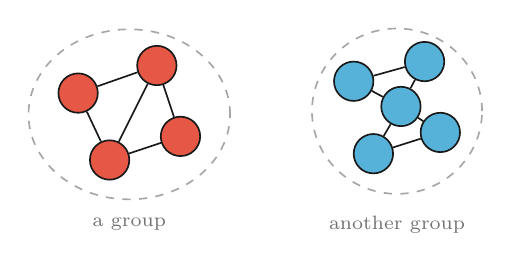
\begin{tikzpicture}[line width=0.6pt,
   nf/.style={circle, draw=ink, fill=clusterA, minimum size=5mm, inner sep=0pt},
   nb/.style={circle, draw=ink, fill=clusterB, minimum size=5mm, inner sep=0pt}]
  % cluster A (left)
  \node[nf](a1) at (0.3,1.05){}; \node[nf](a2) at (1.30,1.40){};
  \node[nf](a3) at (1.60,0.50){}; \node[nf](a4) at (0.70,0.20){};
  \draw[ink] (a1)--(a2) (a1)--(a4) (a2)--(a3) (a3)--(a4) (a2)--(a4);
  \draw[soft, dashed] (0.95,0.78) ellipse (1.28 and 1.08);
  \node[mid, font=\fontsize{7.5}{8}\selectfont] at (0.95,-0.62) {a group};
  % cluster B (right)
  \node[nb](b1) at (3.80,1.20){}; \node[nb](b2) at (4.70,1.45){};
  \node[nb](b3) at (4.90,0.55){}; \node[nb](b4) at (4.05,0.28){}; \node[nb](b5) at (4.40,0.88){};
  \draw[ink] (b1)--(b5) (b2)--(b5) (b3)--(b5) (b4)--(b5) (b1)--(b2) (b3)--(b4);
  \draw[soft, dashed] (4.35,0.82) ellipse (1.08 and 1.05);
  \node[mid, font=\fontsize{7.5}{8}\selectfont] at (4.35,-0.62) {another group};
\end{tikzpicture}}

% --- colour wheel: twelve colours = twelve notes ---------------------------
\newcommand{\colourwheel}{%
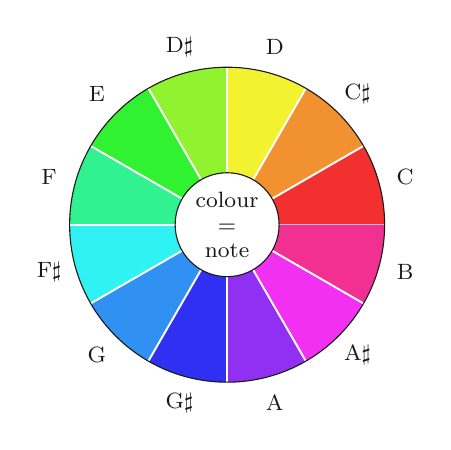
\begin{tikzpicture}[line width=0.4pt, font=\fontsize{7.6}{8}\selectfont]
  \def\R{2.0}
  \foreach \i/\note in {0/C,1/{C\(\sharp\)},2/D,3/{D\(\sharp\)},4/E,5/F,6/{F\(\sharp\)},7/G,8/{G\(\sharp\)},9/A,10/{A\(\sharp\)},11/B}{
    \fill[hue\i] (0,0) -- ({\i*30}:\R) arc ({\i*30}:{\i*30+30}:\R) -- cycle;
    \draw[white, line width=0.7pt] (0,0) -- ({\i*30}:\R);
    \node[ink] at ({\i*30+15}:{\R+0.34}) {\note};
  }
  \draw[ink] (0,0) circle (\R);
  \fill[white] (0,0) circle (0.66);
  \draw[ink] (0,0) circle (0.66);
  \node[ink, align=center, font=\fontsize{8}{9}\selectfont] at (0,0) {colour\\$=$\\note};
\end{tikzpicture}}

% --- shake = chime ----------------------------------------------------------
\newcommand{\shakefig}{%
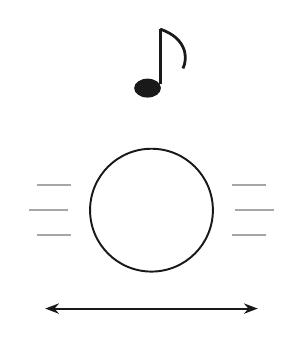
\begin{tikzpicture}[line width=0.7pt]
  \draw[ink] (0,0) circle (0.78);
  % shake ghost lines
  \foreach \s in {-1,1}{
    \draw[soft] (\s*1.02,0.32) -- (\s*1.46,0.32);
    \draw[soft] (\s*1.06,0)   -- (\s*1.56,0);
    \draw[soft] (\s*1.02,-0.32)-- (\s*1.46,-0.32);
  }
  % shake arrow
  \draw[ink,{Stealth[length=5pt]}-{Stealth[length=5pt]}] (-1.35,-1.25) -- (1.35,-1.25);
  % chime — an eighth note above
  \fill[ink] (-0.05,1.55) ellipse (0.17 and 0.12);
  \draw[ink, line width=1.0pt] (0.11,1.60) -- (0.11,2.30);
  \draw[ink, line width=1.0pt] (0.11,2.30) .. controls (0.46,2.18) and (0.46,1.92) .. (0.40,1.80);
\end{tikzpicture}}

% --- spin = sustained pad ---------------------------------------------------
\newcommand{\spinfig}{%
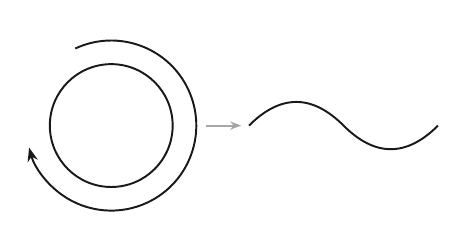
\begin{tikzpicture}[line width=0.7pt]
  \draw[ink] (0,0) circle (0.78);
  % rotation arrow around the orb
  \draw[ink,-{Stealth[length=5pt]}] (115:1.08) arc (115:-165:1.08);
  % a long, held wave = the sustained pad
  \draw[soft,-{Stealth[length=4pt]}] (1.2,0) -- (1.65,0);
  \draw[ink] (1.75,0) .. controls (2.15,0.40) and (2.55,0.40) .. (2.95,0)
                      .. controls (3.35,-0.40) and (3.75,-0.40) .. (4.15,0);
\end{tikzpicture}}

% --- genealogy timeline -----------------------------------------------------
\newcommand{\timelinefig}{%
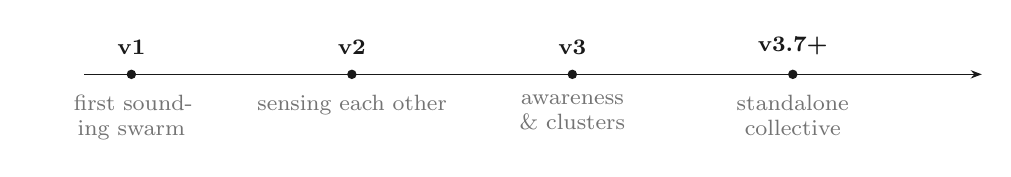
\begin{tikzpicture}[line width=0.5pt, font=\fontsize{7.6}{9}\selectfont]
  \draw[ink,-{Stealth[length=4pt]}] (0,0) -- (11.4,0);
  \foreach \x/\v/\c in {0.6/v1/{first sounding swarm}, 3.4/v2/{sensing each other}, 6.2/v3/{awareness \& clusters}, 9.0/{v3.7+}/{standalone collective}}{
    \fill[ink] (\x,0) circle (0.06);
    \node[anchor=south, ink, font=\fontsize{8}{9}\selectfont\bfseries] at (\x,0.12) {\v};
    \node[anchor=north, mid, text width=24mm, align=center] at (\x,-0.14) {\c};
  }
\end{tikzpicture}}

% ===========================================================================
\begin{document}
\begin{tikzpicture}[remember picture, overlay]

% ---- fold / crop guides ---------------------------------------------------
\foreach \c in {1,2,3,4,5}{
  \draw[hair, dash pattern=on 2pt off 2pt]
    ($(current page.north west)+(\c*148mm,-6mm)$) -- ($(current page.north west)+(\c*148mm,-414mm)$);
}
\draw[hair, dash pattern=on 2pt off 2pt]
  ($(current page.north west)+(6mm,-210mm)$) -- ($(current page.north west)+(882mm,-210mm)$);
\foreach \c in {0,1,2,3,4,5,6}{
  \draw[soft,line width=0.4pt] ($(current page.north west)+(\c*148mm,0)$) -- ++(0,-4mm);
  \draw[soft,line width=0.4pt] ($(current page.south west)+(\c*148mm,0)$) -- ++(0,4mm);
}

% =====================  TOP ROW  ===========================================

% --- (0,0) COVER -----------------------------------------------------------
\panel{0}{0}{%
  \vfill
  \begin{center}
    \orbglyph{1.9}\\[10mm]
    {\fontsize{46}{46}\selectfont\bfseries nOdes}\\[3mm]
    {\fontsize{15}{18}\selectfont\addfontfeatures{LetterSpace=8.0}\MakeUppercase{Obstruction Manual}}\\[7mm]
    {\fontsize{11}{15}\selectfont\itshape an open intuitive score\\for a swarm of light}
  \end{center}
  \vfill
  {\color{hair}\hrule height 0.4pt}\medskip
  \fine{This is not a step-by-step guide for replication, but a prompt for reinterpretation. Open it fully as a poster, or fold it to A5. The reverse is left blank — for your own notes.}
}

% --- (1,0) THE INSTRUMENT --------------------------------------------------
\panel{1}{0}{%
  \kicker{The instrument}\par\smallskip
  \panelhead{A constellation\\you play together}\par\medskip
  \body{nOdes is a swarm of spherical, handheld \emph{orbs} — each a self-contained wireless device with motion sensing, twelve icosahedrally-arranged LEDs, audio and battery power.}
  \body{Ten to twenty-four people play it at once, shaping a shared harmonic environment by rotating, shaking, passing and clustering their orbs. The swarm responds to the crowd — not the other way around.}
  \vfill
  \begin{center}
    \qrcode[height=20mm]{https://nodes.invalid/repository}\\[2mm]
    \fine{repository — release pending}
  \end{center}
}

% --- (2,0) ANATOMY ---------------------------------------------------------
\panel{2}{0}{%
  \kicker{Anatomy of an orb}\par\smallskip
  \begin{center}\vspace{1mm}
\includegraphics[height=146mm]{../NIME/Figures/orb-exploded-final}\end{center}
  \vfill
  \obnote{Shown exploded, not in assembly order. How the parts fit — and which you truly need — is left for you to work out.}
}

% --- (3,0) SOFTWARE & AUTHORING --------------------------------------------
\panel{3}{0}{%
  \kicker{Software \& authoring}\par\smallskip
  \begin{center}\vspace{1mm}
\includegraphics[width=\linewidth]{{../NIME/Figures/SystemDiagram_nOdes.drawio}.pdf}\end{center}
  \smallskip
  \body{Orbs stream motion to a server over Wi-Fi at 50\,Hz. A C\texttt{++} server reduces the whole swarm to a few collective measures and hands them on as light and sound.}
  \rulein
  {\fontsize{12}{15}\selectfont\bfseries Authoring an experience}\par\smallskip
  \body{The orbs stay sealed — their firmware travels wirelessly, \emph{over the air}, so you rarely open one. But the art lives on the \emph{server}. A new piece is a short \textbf{Python} script over the live state of the whole swarm: read motion and clustering, \emph{prompt} the crowd (``find your colour'', ``make one group''), measure how the collective responds, and answer in light and sound on the orbs.}
  \vfill
  \obnote{Omitted by design: the exact packet layout, slot allocation and firmware. Rediscover them, or ask the repository.}
}

% --- (4,0) PHENOMENOLOGY ---------------------------------------------------
\panel{4}{0}{%
  \kicker{Phenomenology of the swarm}\par\smallskip
  \lede{The swarm is a single shifting body made of many hands.}\par\medskip
  \body{No one plays a melody; everyone tends a weather. Structure and chaos take turns. You feel part of a collective before you understand how.}
  \body{The feedback loop runs from sensor to collective metric to light and sound on the orbs themselves — not through loudspeakers in the room. It grows out of swarm robotics and community music-making: an instrument that needs other people.}
  \rulein
  \obnote{This manual is intentionally incomplete. Following the Obstruction Manual method, it withholds steps to leave room for your own making. The gaps are the invitation.}
}

% --- (5,0) GENEALOGY -------------------------------------------------------
\panel{5}{0}{%
  \kicker{Where it came from}\par\smallskip
  \body{Four eras, each adding a sense.}
  \vfill
  \begin{center}\timelinefig\end{center}
  \vfill
  \body{First sound; then mutual awareness; then collective behaviour; then the resilience to keep playing when the network falls quiet.}
}

% =====================  BOTTOM ROW — HOW YOU PLAY IT  =======================

% --- (0,1) CLUSTERING ------------------------------------------------------
\panel{0}{1}{%
  \kicker{1 · Clustering}\par\smallskip
  \panelhead{The swarm finds\\its groups}\par\medskip
  \begin{center}\vspace{2mm}\clusternet\vspace{2mm}\end{center}
  \body{Bring orbs close and they form a group. The swarm works out its own clusters from who is near whom — and \emph{each group takes on a colour}. This is where the music begins, so start here.}
}

% --- (1,1) COLOUR = NOTE ---------------------------------------------------
\panel{1}{1}{%
  \kicker{2 · Colour {\normalfont$=$} note}\par\smallskip
  \begin{center}\vspace{1mm}\colourwheel\end{center}
  \smallskip
  \body{Each colour is a note. A group glows its colour and sounds that note — so a \emph{different cluster sings a different note}. Twelve colours, twelve notes, around the wheel.}
}

% --- (2,1) SHAKE = CHIME ---------------------------------------------------
\panel{2}{1}{%
  \kicker{3 · Shake {\normalfont$=$} chime}\par\smallskip
  \panelhead{Shake an orb}\par\medskip
  \begin{center}\vspace{6mm}\shakefig\vspace{8mm}\end{center}
  \body{A sharp shake rings a \emph{chime} — a bright, percussive transient that sounds over the cluster's note. The harder the swarm moves, the more it sparkles.}
}

% --- (3,1) SPIN = SUSTAINED PAD --------------------------------------------
\panel{3}{1}{%
  \kicker{4 · Spin {\normalfont$=$} pad}\par\smallskip
  \panelhead{Spin an orb}\par\medskip
  \begin{center}\vspace{6mm}\spinfig\vspace{8mm}\end{center}
  \body{Keep an orb turning and its note swells into a \emph{sustained pad} — a long, held voice. Hold the motion, hold the sound; let it fall still and the pad fades.}
}

% --- (4,1) TROUBLESHOOTING -------------------------------------------------
\panel{4}{1}{%
  \kicker{When it resists}\par\smallskip
  \body{\textbf{An orb won't join?} It is waiting for the access point. Power-cycle it close to the AP.}
  \body{\textbf{One orb glows the wrong colour in a big swarm?} Past about twenty-five orbs the marginal orb starves of downlink. It is coverage, not a fault — move the access point, or thin the crowd.}
  \body{\textbf{Silence at rest?} That is correct. The swarm sings on movement and change, not on stillness.}
  \vfill
  \begin{center}
    \qrcode[height=18mm]{https://nodes.invalid/troubleshooting}\\[2mm]
    \fine{runbook — release pending}
  \end{center}
}

% --- (5,1) CREDITS ---------------------------------------------------------
\panel{5}{1}{%
  \kicker{Credits}\par\smallskip
  \body{Tom Didiot-Cook, Simon Jones, Johanna Blee, Razanne Abu-Aisheh, Sabine Hauert\\\fine{University of Bristol}}
  \body{Nadine Meertens, Ophelia Deroy\\\fine{LMU München}}
  \rulein
  \fine{Funded by the Horizon Europe EMERGE Project (101070918) and UKRI grant 10038942.}
  \fine{Synthesis via \emph{Cellular Au-Tonnetz} (T. Didiot-Cook, 2025).}
  \vfill
  \begin{center}
    \qrcode[height=18mm]{https://doi.org/10.1007/978-3-031-90167-6_4}\\[2mm]
    \fine{Cellular Au-Tonnetz — doi.org/10.1007/978-3-031-90167-6\_4}
  \end{center}
  \medskip
  \fine{Manual after Merendino, Masu \& Lepri, \emph{The Obstruction Manual}, NIME 2026.\\ \textcopyright\ 2026 the authors · CC BY 4.0}
}

\end{tikzpicture}
\end{document}
